\section{Conceptual design and justification of the design}

In order to set the right design goals and milestones during the semester, adequately estimate the workload and organize the working process in the most effective way, we needed to: analyze the initial design conditions and restrictions, roughly formulate the implementation blocks along with respective skill-sets of all project members and - after that - write down the most suitable working program. Both steps are described in detail below.

\subsection{Initial design conditions} \label{chap:design_cond}
The main question to answer was to grasp and implement using the knowledge we had acquired plus the logic behind the "how do we build a robot that should drive in the labyrinth and be able to make intelligent decisions (turns) based on the observations (made by sensors)"?

\noindent 
There are some predefined conditions and tools that we used as a starting point in answering this question: 

\begin{itemize}
    \item Geometric constraints\\ 
    As was mentioned in the previous section, the geometric parameters of the maze in our case were as following: 8x8 identical squares with a side of 16cm. Therefore, our "mouse" was logically required to be smaller than 16cm in width and length, ideally the size that would allow it to move freely while performing any type of movement within the maze (therefore leaving at least 2-3 centimeters of distance to the surrounding walls)
    \item Power supply\\
    According to the unified formal requirements of the Micromouse competition, the robot should be autonomous, which infers carrying it's own power supply in form of a standard 9V battery.
    \item Sensing the environment\\
    The initial condition in regards to sensing simply states that the robot should be able to perceive the environment and make informed decisions about the next movement (moving straight or turning in one of the directions - the turn angle was set to be fixed at 90 degrees in order to simplify the design) based on the analysis of the information received from the sensors. The sensor type that is the most efficient for the cause - simple infrared proximity sensor. We had an option to either order the desired amount of sensors or to build them ourselves.
    \item Motors\\
    In order for the "mouse" to move, we were provided with predefined 2619-SR-IE2-16 motors and sets of wheels of different diameter.
    \item Microcontroller\\
    Initially, for the educational purposes and in order to gain some knowledge in configuring and setting up the microcontroller to control the needed peripherals, a pair of dsPIC30F4011 microcontrollers was provided. Appropriate for the goal task microcontroller was decided to be chosen later. Overall, it had to have all required pins and interfaces, such as:\\
    - PWM outputs for the motor control\\
    - analog inputs to receive data from sensors\\
    - enough extra pins to connect peripherals (such as LEDs)\\
    - flexible and convenient pin mapping in order to satisfy the geometric constraints
    \item PCB\\
    The printed circuit board for the robot was to be designed independently, according to all the aforementioned conditions.
    \item Casing\\
    In order for all of the components (such as the board, the motors and the battery) to hold together in one single "mouse" unit, it was set that a custom casing must be designed and printed.
\end{itemize}

Based on those conditions and also tools and devices provided, we came up with the implementation plan, which can be seen in detail in the next part.

\subsection{Work program and Gantt chart}
In the below Fig. \ref{fig:gantt}, we describe our planned stages within a Gantt chart.

\begin{figure}[H]
    \centering
    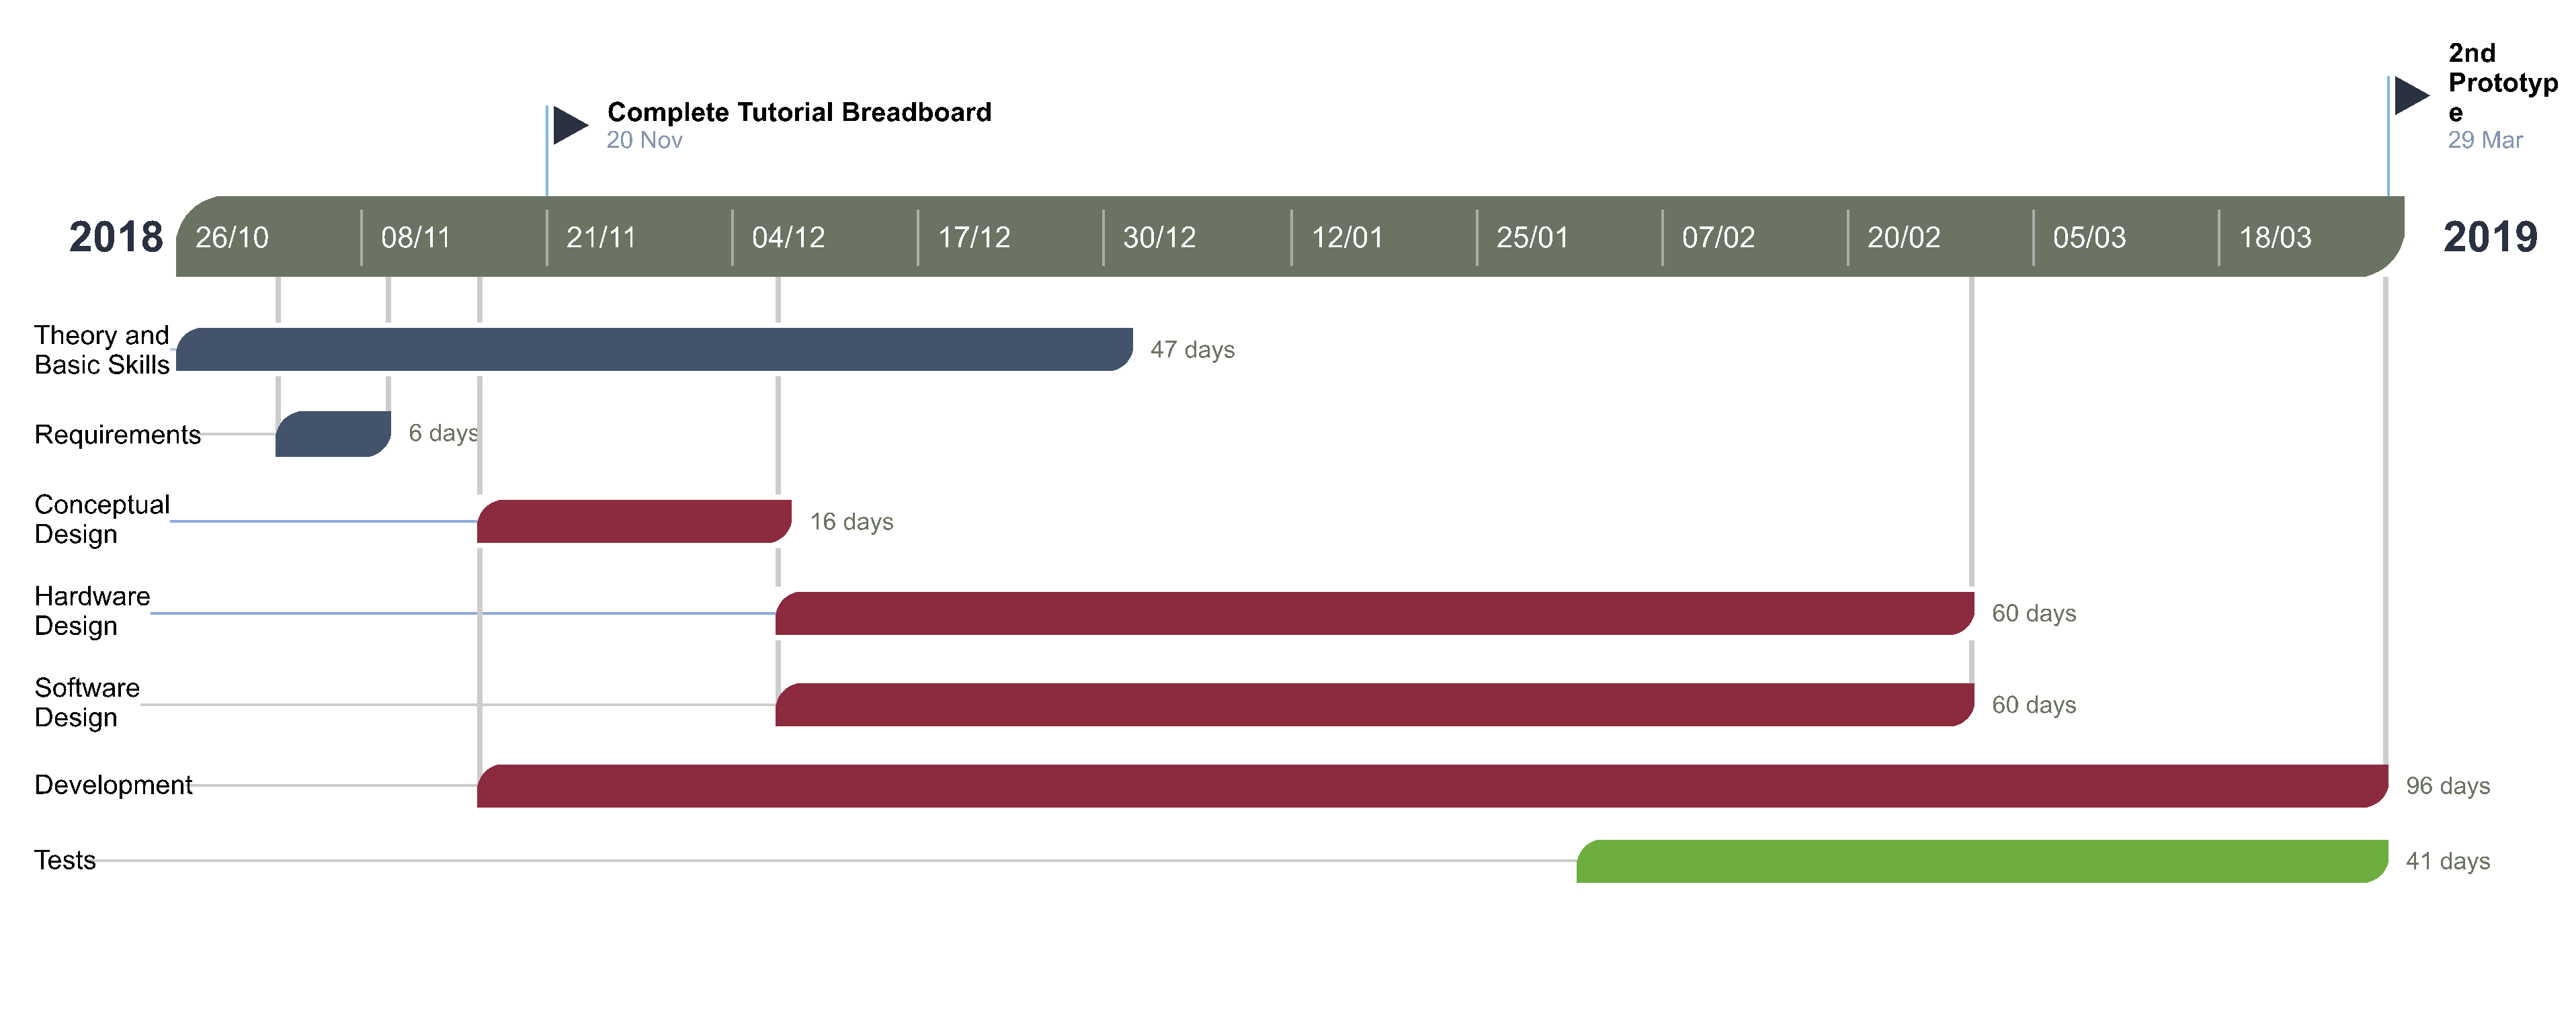
\includegraphics[width=1\textwidth]{figures/micromouse-gantt.png}
    \caption{Gantt chart of our progress}
    \label{fig:gantt}
\end{figure}

\noindent
In the first half of the semester we started off with a basic introduction to electrical engineering. By using the microcontroller dsPIC30F4012 we followed a practical course and learned to use the Microchip MPLABX environment in order to create and simulate the code for the software of the micromouse.

\noindent
The practial course was comprised of the following topics:
\begin{itemize}
    \item Digital I/O
    \item Interrupts
    \item PWM
    \item UART
    \item Quadrature Encoders
    \item Analogue Inputs
\end{itemize}

\noindent
During the practial course we applied our learnings onto a breadboard. Which can be seen in figure \ref{fig:breadboard}. By doing this we got an idea of what kind of electronic parts we will need to get accustomed with for the creation of the final micromouse. Our acquired knowledge will be described in more detail in the next chapter.

\begin{figure}[H]
    \centering
    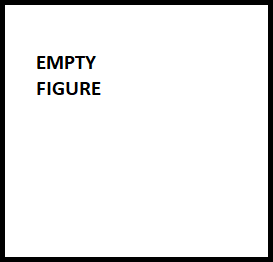
\includegraphics[width=0.2\textwidth]{figures/filler.png}
    \caption{\textcolor{red}{First completed breadboard}}
    \label{fig:breadboard}
\end{figure}

\noindent
While going through the practical course, we fetched all the requirements we would need during the preparations of building the micromouse. All of them are described in the previous chapter \ref{chap:design_cond} \\

\noindent
The former idea of splitting us students into two separate groups was canceled because it took us too long to complete the basic introduction (as it was initially planned) plus the fact that we all were inexperienced in electrical engineering. Instead we formed two teams: One was responsible for the hardware the other one for the software design. \\
So after all requirements were known and the conceptual design phase was completed, we started with designing the hardware and software. Both are described in more detail in the chapters \ref{chap:hardware} and \ref{chap:software} respectively. \\
In order to construct a PCB with all the parts we need, we are using Autodesk Eagle. For writing the software we are using the MPLABX environment. \\

\noindent
The testing part concludes the overall development stage. And because testing is such a crucial element during a development, especially when designing hardware is a part of it, every step has to be done with caution. Hence, a failure of an electrical compound can easily lead to a broken part, which will result in unnecessary costs and time delays. The test results can be found in chapter \ref{chap:tests}. \\

\textcolor{red}{I would suggest to fit here the part with "design decisions based on the aforementioned conditions (justification)"
\textit{ This is where I'm a bit lost. We could include some "ideal" version of this chart here, but where exactly should we describe all the changes in planning and organization and why they had to be done at each stage of building the prototype and the final version of the mouse?  Should it be described here? Or later in the "problems and challenges"?
Also I think maybe here we should talk about all the initial learning stage we had to go through in the first half of the praktikum (maybe devote a subsection for this here or later in the report)}}

